\documentclass{article}
	\usepackage{graphicx}

	\begin{document}

	\title{HW/SW Entwurfssprachen am Beispiel System-C}
	\author{Florian Zaruba, Thomas Weber}

	\maketitle

	%\begin{abstract}
	%The abstract text goes here.
	%\end{abstract}

	\section{HW/SW Design Languages}
	tba
	\section{What is SystemC}
	tba
	  \subsection{History}
	  tba
	  \subsection{Benefits}
	  tba
	  \subsection{Drawbacks}
	  tba
	  \subsection{SysC vs. C}
	  tba
	  \subsection{SysC vs. VHDL}

	\section{Automatic Partitioning}
	  \subsection{What is Partitioning?}
	  Partitioning means the separation of hardware and software parts in focus on hardware/software co-design.
	  Traditionally the hardware part of an embedded system is written in VHDL \textit{(more present in Europe)} or Verilog \textit{(more present in the USA)} while the software part is written in \textit{assembly}, \textit{C} or \textit{C++}.
	  The common design-flow (depicted in \ref{fig:flow}) shows that, after partitioning the design in hardware and software,  it is necessary to do all steps before the re-design 
	    \begin{figure}[tp]
	      \centering
	      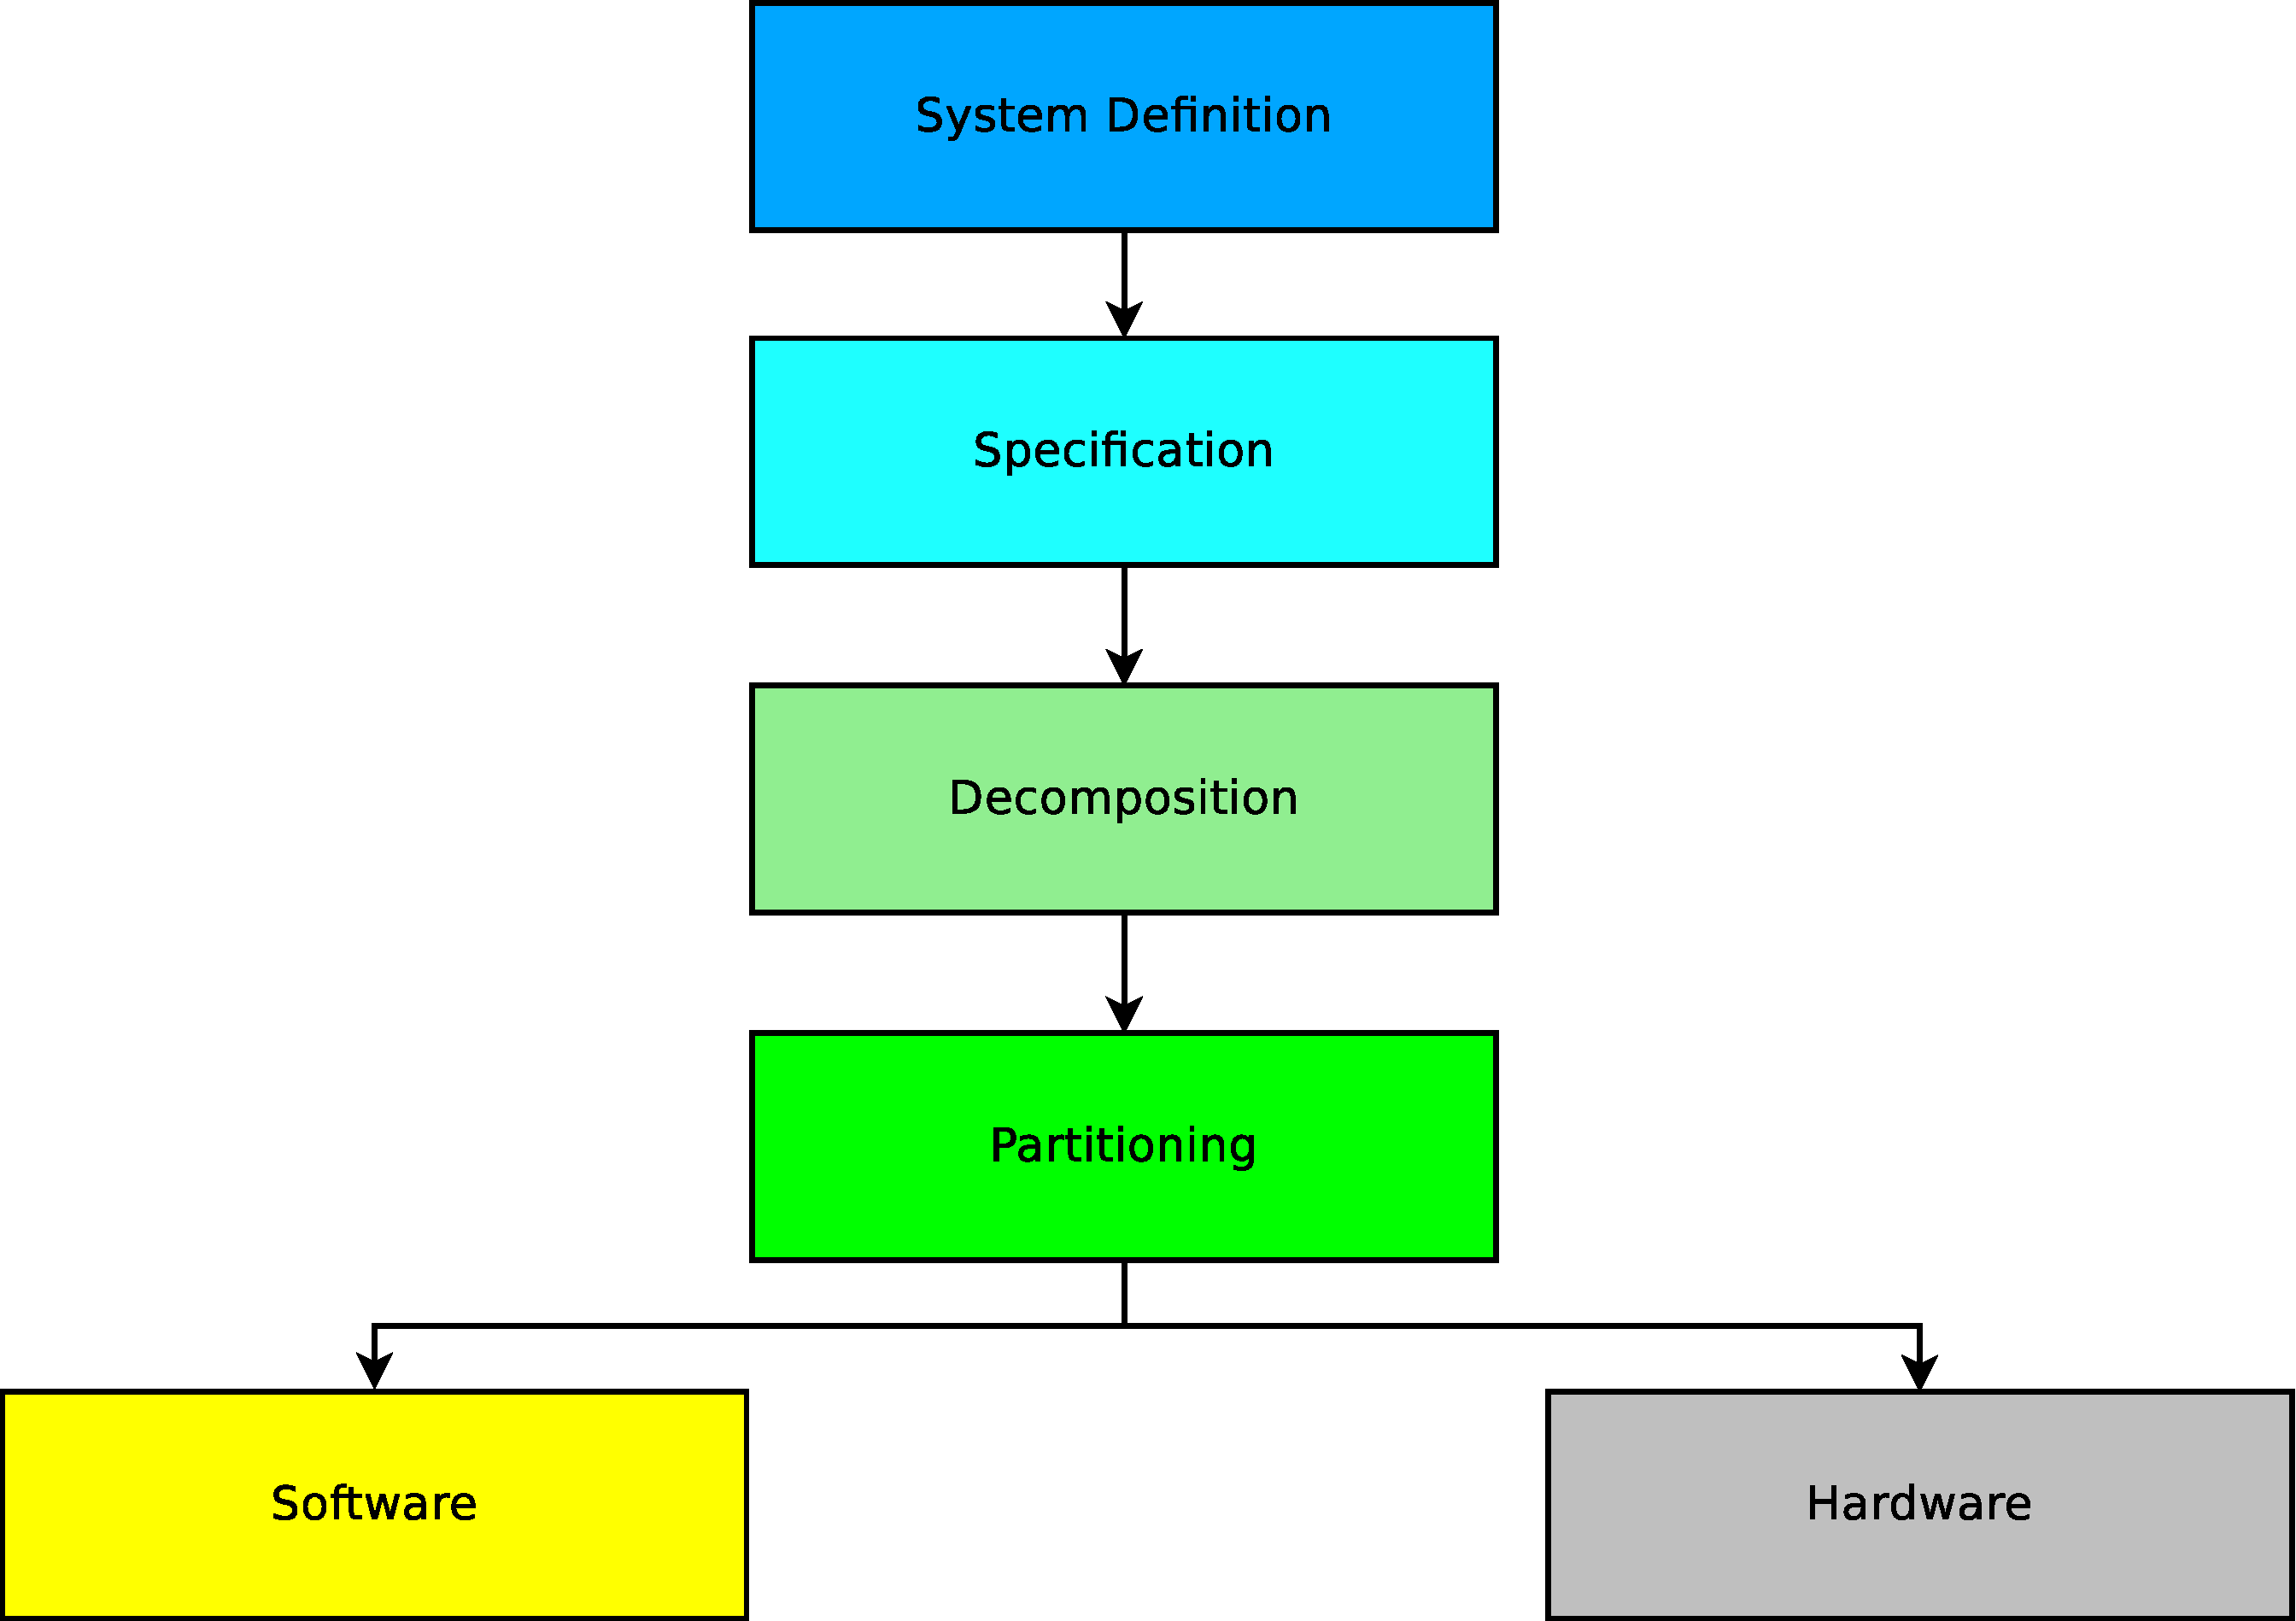
\includegraphics[scale=0.18]{../pictures/flow.pdf}
	      \caption{Design flow \textit{(c.f. Hardware Modelling VO)}.}
	      \label{fig:flow}
	    \end{figure}  
	  \subsection{}
	  
	\section{Tools}

	\section{Users}

\end{document}
